One of the most established and popular tools that can generate documentation from C++ sources is Doxygen. And when I say "established", I mean it: the first version was released by Dimitri van Heesch in October 1997. Since then, it has grown immensely, and it is actively supported by over 180 contributors to its repository (\url{https://github.com/doxygen/doxygen}).

Doxygen can produce documentation in the following formats:

\begin{itemize}
\item 
HyperText Markup Language (HTML)

\item 
Rich Text Format (RTF)

\item 
Portable Document Format (PDF)

\item 
Lamport's TeX (LaTeX)

\item 
PostScript (PS)

\item 
Unix manual (man pages)

\item 
Microsoft Compiled HTML Help (CHM)
\end{itemize}

If you decorate your code with comments providing additional information in the format specified by Doxygen, it will be parsed to enrich the output file. What's more, the code structure will be analyzed to produce helpful charts and diagrams. The latter is optional, as it requires an external Graphviz tool (\url{https://graphviz.org/}).

The developer should first answer the following question: Do users of the project just get the documentation or will they generate it themselves (perhaps when they build from source)? The first option implies that documentation is shipped with the binaries, available online, or (less elegantly) checked in with the source code into the repository.

The answer matters, because if we want users to generate documentation during the build, they will need the dependencies present in their system. This isn't too large a problem since Doxygen is available through most package managers (as well as Graphviz), and all that's needed is a simple command, such as this one for Debian:

\begin{tcblisting}{commandshell={}}
apt-get install doxygen graphviz
\end{tcblisting}

There are also binaries available for Windows (check the project's website).

To summarize: generate documentation for users or handle adding the dependencies if needed. This is covered in Chapter 7, Managing Dependencies with CMake, so we won't repeat the steps here. Note that Doxygen is built with CMake, so you can easily compile it from source as well.

When Doxygen and Graphviz are installed in the system, we can add the generation to our project. Unlike as suggested by online sources, this isn't as hard or involved as we might think. We don't need to create external configuration files, provide paths to the doxygen executable, or add custom targets. Since CMake 3.9, we can use the doxygen\_add\_docs() function from FindDoxygen find-module, which sets the documentation target up.

The signature looks like this:

\begin{lstlisting}[style=styleCMake]
doxygen_add_docs(targetName [sourceFilesOrDirs...]
	[ALL] [USE_STAMP_FILE] [WORKING_DIRECTORY dir]
	[COMMENT comment])
\end{lstlisting}

The first argument specifies the target name, which we'll need to build explicitly with the -t argument to cmake (after generating a build tree), as follows:

\begin{tcblisting}{commandshell={}}
cmake --build <build-tree> -t targetName
\end{tcblisting}

Or, we can always have it be built by adding the ALL argument (usually not necessary). Other options are pretty self-explanatory, except maybe USE\_STAMP\_FILE. This allows CMake to skip regeneration of documentation if none of the source files have changed (but requires sourceFilesOrDirs to only contain files).

We'll follow the practice from previous chapters and create a utility module with a helper function (so that it can be reused in other projects), as follows:

\begin{lstlisting}[style=styleCMake]
# chapter-10/01-doxygen/cmake/Doxygen.cmake

function(Doxygen input output)
	find_package(Doxygen)
	if (NOT DOXYGEN_FOUND)
		add_custom_target(doxygen COMMAND false
			COMMENT "Doxygen not found")
		return()
	endif()
	set(DOXYGEN_GENERATE_HTML YES)
	set(DOXYGEN_HTML_OUTPUT
		${PROJECT_BINARY_DIR}/${output})
		
	doxygen_add_docs(doxygen
		${PROJECT_SOURCE_DIR}/${input}
		COMMENT "Generate HTML documentation"
	)
endfunction()
\end{lstlisting}

The function accepts two arguments—input and output directories—and will create a custom doxygen target. Here's what happens:

\begin{enumerate}
\item 
First, we'll use CMake's built-in Doxygen find-module to figure out if Doxygen is available in the system.

\item 
If it isn't available, we'll create a dummy doxygen target that will inform the user and run a false command, which (on Unix-like systems) returns 1, causing the build to fail. We terminate the function at that time with return().

\item 
If Doxygen is available, we'll configure it to generate HTML output in the provided output directory. Doxygen is extremely configurable (find out more in the official documentation). To set any option, just follow the example by calling set() and prepend its name with DOXYGEN\_.

\item 
Set up the actual doxygen target: all the DOXYGEN\_ variables will be forwarded to Doxygen's configuration file, and documentation will be generated from the provided input directory in the source tree.
\end{enumerate}

If your documentation is to be generated by users, Step 2 should probably involve installing the necessary dependencies instead.

To use this function, we can add it to the main listfile of our project, as follows:

\begin{lstlisting}[style=styleCMake]
# chapter-10/01-doxygen/CMakeLists.txt

cmake_minimum_required(VERSION 3.20.0)
project(Doxygen CXX)
enable_testing()
list(APPEND CMAKE_MODULE_PATH "${CMAKE_SOURCE_DIR}/cmake")
add_subdirectory(src bin)

include(Doxygen)
Doxygen(src docs)
\end{lstlisting}

Not difficult at all. Building the doxygen target generates HTML documentation that looks like this:

\begin{center}
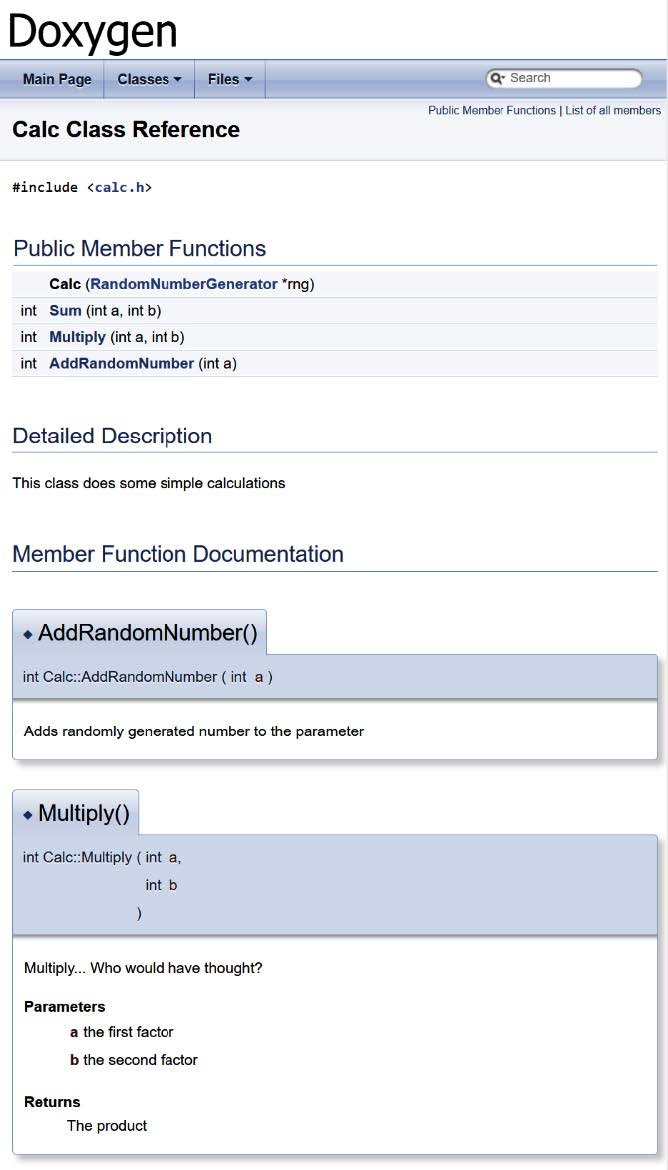
\includegraphics[width=0.8\textwidth]{content/3/chapter10/images/1.jpg}\\
Figure 10.1 – Class reference generated with Doxygen
\end{center}

The additional description you can see in Member Function Documentation is added by prepending the method with an appropriate comment in the header file, as follows:

\begin{lstlisting}[style=styleCXX]
// chapter-10/01-doxygen/src/calc.h (fragment)

/**
Multiply... Who would have thought?
@param a the first factor
@param b the second factor
@result The product
*/
int Multiply(int a, int b);
\end{lstlisting}

This format is known as Javadoc. It is important to open the comment block with double asterisks: /**. More information can be found in the description of Doxygen's docblocks (see the link in the Further reading section).

As mentioned earlier, if Graphviz is installed, Doxygen will detect it and generate dependency diagrams, as illustrated here:

\begin{center}
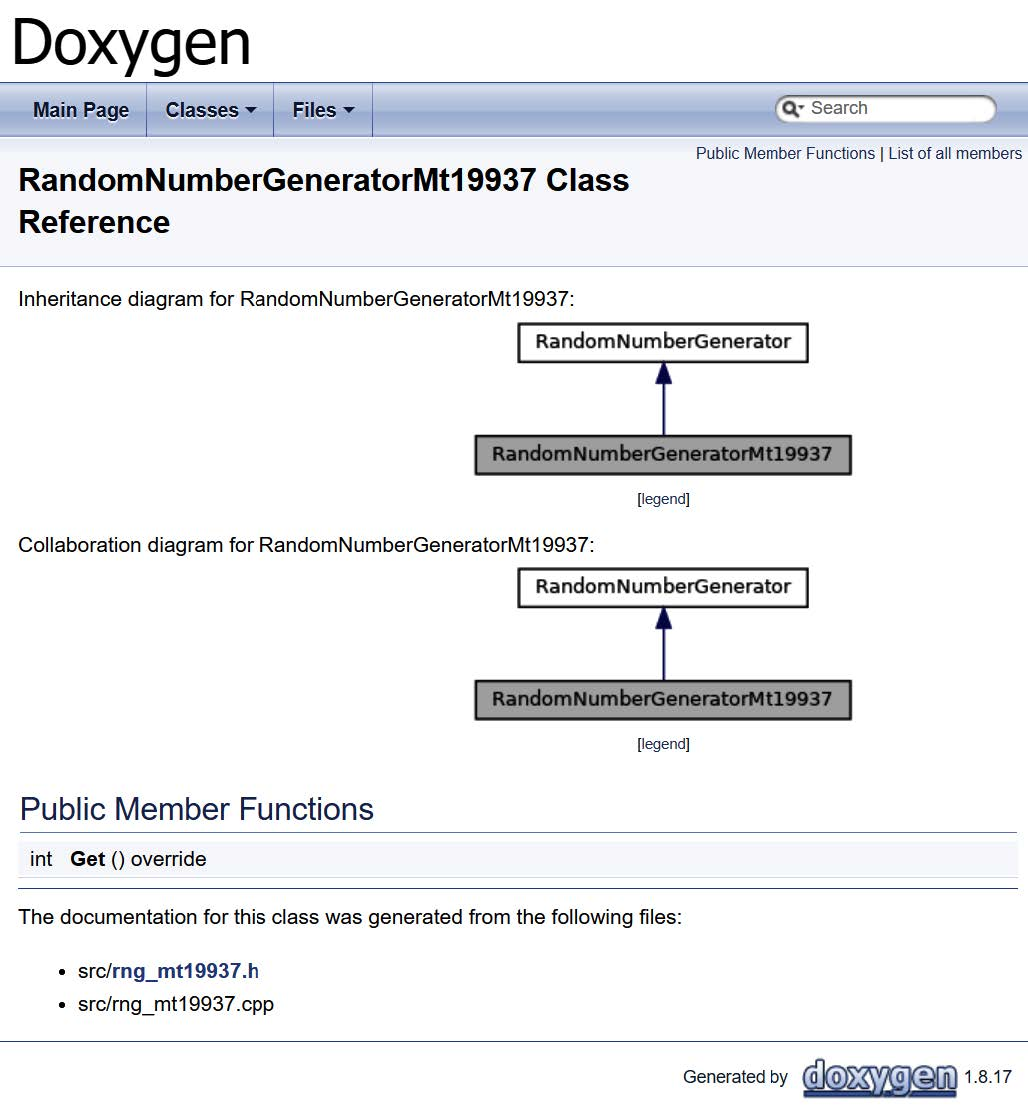
\includegraphics[width=0.8\textwidth]{content/3/chapter10/images/2.jpg}\\
Figure 10.2 – Inheritance and collaboration diagrams generated by Doxygen
\end{center}

By generating documentation straight from the source, we create a mechanism to quickly update it with any code changes happening throughout the development cycle. Also, any missed updates in the comments have a chance of being spotted during the code review.

Many developers will complain that the design offered by Doxygen is dated, which makes them hesitant to present generated documentation to their customers. Don't worry— there's an easy solution to this problem.









